\chapter{Introduction} \label{intro}
The trustworthiness and assurance that a system will perform as anticipated needs heavy testing. When a software carries the critical responsibility of examining the human body, administering medication to patients, saving millions of lifes, and conversely, the tiniest bug or error in the implementation process could have derive into seriour consequences for individuals' well-being. This happens when there are problems with how the system works, whether we expected them or not. It's also influenced by things like the environment it's in, the risks it might face, and people who might want to cause harm. To feel sure about the system, we need to pay attention to its main qualities and collect good evidence that it's doing what we want it to do.

Medical software is tricky to make sure it's reliable. The way it's built is very sensitive, so it might not be possible for the users to check how it works. But without the implementation details, it's hard to trust it, especially for something as important as medical software.

Under this context, we want to explore the feasibility of applying assurance cases over a medical software from the beginning of the development. With selected arguments and evidences, we want to show to the domain experts that the software delivers correct outputs when used for its intented use/purpose in its intended environment, and within its assumed operating assumptions.

\section{Objective} \label{obj}
In this study, we present the results of applying assurance cases during the development of medical software to enhance stakeholders' confidence in this software. The software, AortaGeomRecon, is a 3D Slicer extension module that aims to semi-automatically construct a 3D model of the Aorta from a patient's chest CT scans. Assurance cases serve as a method for providing assurance for a system by presenting arguments to justify claims about the system, based on evidence regarding its design, development, and tested behavior.

This case study first introduces the challenge of Organ/Aorta Segmentation and explores existing solutions, which might require time and effort from domain experts. Then, we outline the workflow and logic of our algorithm, as well as the working environment for using this module within 3D Slicer. Finally, we discuss our assurance cases, including selected arguments and evidence. This discussion aims to explain how these selected elements enabled us to cultivate confidence in the reliability of the medical software.

\section{Background} \label{bg}

\subsection{Aorta}
Aorta is the largest artery that carries blood from the heart to the circulatory system. It has a cane-liked shape with Ascending aorta, Aortic arch and Descending aorta. 

\begin{figure}[ht]
    \centering
    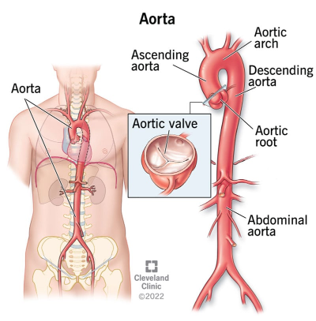
\includegraphics[width=0.4\textwidth]{figures/Intro/Aorta.png}
    \caption[Aorta]{Aorta}
    \label{fig_aorta}
\end{figure}

Aorta segmentation in CT scans is important for:
\begin{itemize}
\item Coarctation of the aorta
\item Aortic calcification quantification
\item To guide the segmentation of other central vessels. 
\end{itemize} ~\\

\subsection{Organ Segmentation}
The definition of the organ boundary or organ segmentation is helpful for the orientation and identification of the regions of interest inside the organ during the diagnostic or treatment procedure. Further, it allows the volume estimation of the organ, such as the aorta.

\begin{figure}[ht]
    \centering
    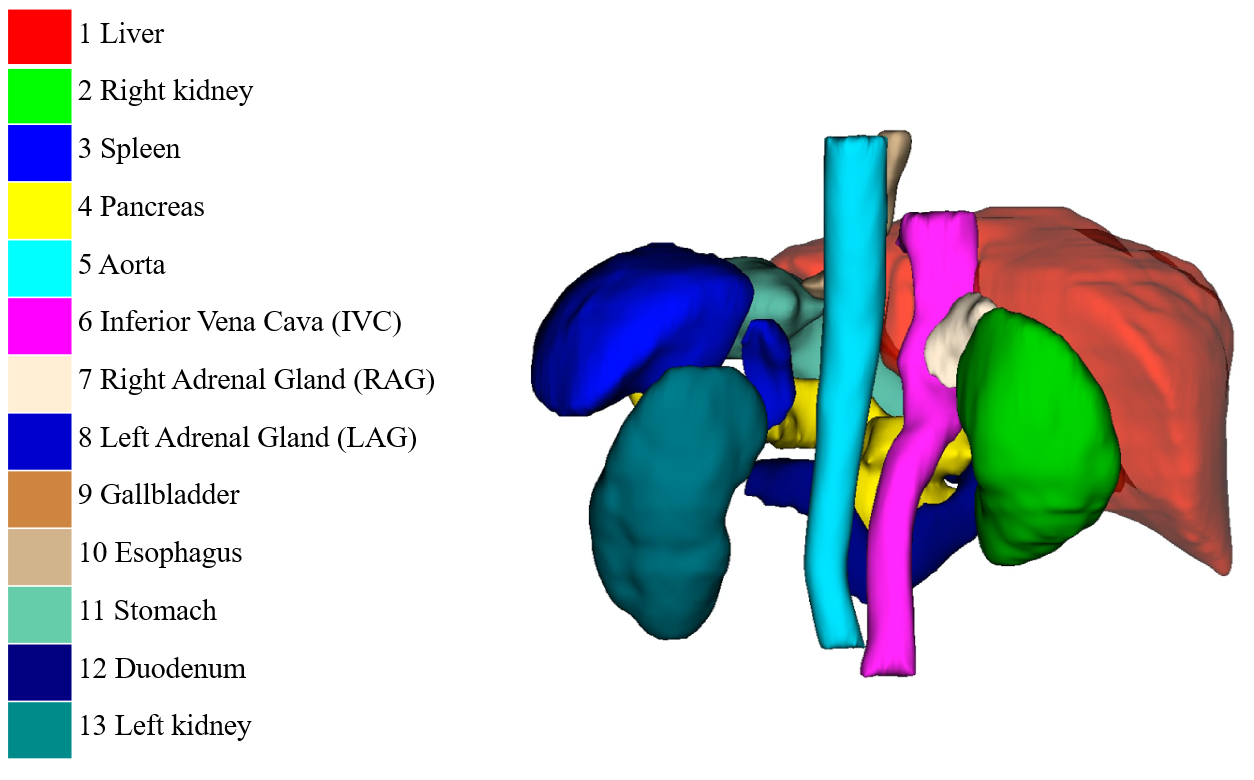
\includegraphics[width=0.7\textwidth]{figures/Intro/segmentation.png}
    \caption[Organ Segmentation]{Organ Segmentation \cite{Ma-2021-AbdomenCT-1K}}
    \label{fig_seg}
\end{figure}

\subsection{Assurance Case}

\begin{figure}[ht]
    \centering
    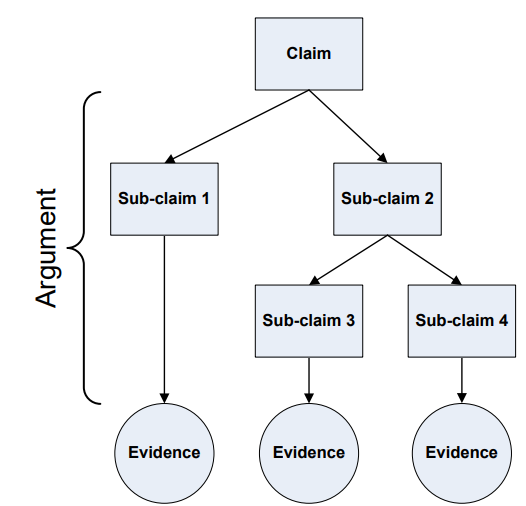
\includegraphics[width=0.45\textwidth]{figures/Intro/ac_diagram.png}
    \caption[Simple Assurance Case Diagram]{Simple Assurance Case Diagram \cite{doi:10.2514/6.2009-1921}}
    \label{fig_ac_diagram}
\end{figure}


An assurance case can be thought of as a specific type of argumentation used in various cases. When building an assurance case, you're essentially making a point that specific evidence backs up a particular statement. The fundamental structure is depicted in Figure \ref{fig_ac_diagram}. So, an assurance case essentially boils down to an organized collection of arguments, backed by a body of evidence, that helps validate the belief in a specific claim.

In a practical sense, creating an assurance case involves beginning with a main claim and then breaking it down into smaller claims through a step-by-step process. These smaller claims, at the most basic level, are supported by concrete evidence.


\section{Thesis Outline} \label{TO}

The thesis is organized into three broad parts. In chapter 2, we introduce our program \progname{} by mentioning the existing methods, the AortaGeomRecon's algorithm overview and step by step  workflow. We explain necessary terms and information to understand how the software functionsfinally, and the 3D Slicer extension module that the user interacts with to get the segmentation result with our algorithm. In chapter 3, we present our assurance case, some sections of our SRS, Design Documents, Module Guide, Algorithm Review, and a test case we developed for verifying and validating the correctness of program \progname{}. Finally, future work is proposed and conclusions are drawn based on the developed assurance case, SRS, segmentation algorithm and 3D Slicer module extension.